%!TEX TS-program = pdflatex
%!TEX root = tesi.tex
%!TEX encoding = UTF-8 Unicode

\chapter{Il Dataset}

Innanzitutto si specifica che con la parola Scarto si indica l'immagine di una carcasse che presenta colla sul fondo, pezzo che, quindi, dovrà essere scartato.
Invece con la parola Conforme si indica l'immagine di una carcassa nella quale la colla è stata depositata correttamente, quindi con fondo pulito.

TODO recap capitolo
In questo capitolo verrà descritto il dataset e quali.


\section{Problematiche Principali}

\subsection{Dataset Piccolo e Sbilanciato}
La prima difficoltà insorge ancora prima di ispezionare le immagini del dataset.
Infatti il dataset non solo comprende solamente 1719 immagini ma è anche fortemente sbilanciato:
\begin{itemize}
    \item 1719 immagini sono Conformi;
    \item 30 immagini sono Scarti.
\end{itemize}

A questo punto è corretto chiedersi se le quasi duemila immagini del dataset siano sufficienti ai nostri scopi.
Nel campo del \textit{Machine Learning}, ed ancora di più in quello del \textit{Deep Learning}, non è raro che il numero di elementi in un dataset sia dell'ordine delle decine di migliaia se non di quello delle centinaia di migliaia.
% TODO aggiungere refs ai dataset
Basti pensare ai dataset più famosi ed usati:
\begin{itemize}
  \item MNIST è un dataset molto famoso contenente $70000$ cifre disegnate a mano appartenenti a $10$ classi in totale.
    È alla stesso tempo sia il punto di partenza dei principianti, perché di facile manipolazione, sia il campo di prova degli esperti, sul quale vengono allenati nuovi modelli prima di passare a compiti più complessi;
  \item CIFAR-10 contiene TODO descrivere 
  \item ImageNet contiene TODO descrivere 
\end{itemize}
%TODO aggiungere immagini esempio??

Ciascuno di questi dataset è stato etichettato\footnote{in inglese \textit{labeled} da \textit{label}, etichetta} a mano.
Ciò significa che ad ogni immagine è stata assegnata, a mano, una classe di appartenenza.
Prendendo in esempio MNIST, se un'immagine raffigura la cifra $7$ allora sarà etichettata con il label \textit{seven} ed apparterrà alla classe di immagini in cui compare la cifra $7$.
Allo stesso modo le immagini di ImageNet hanno etichette come \textit{dog}, \textit{cat}, \textit{bird}, \textit{car}, \textit{bike}, ecc... %TODO forma corretta??
Il nostro dataset, come già illustrato, contiene due classi: Conforme e Scarto.

Sembrerebbe che possedere 2000 immagini appena renda impossibile applicare algoritmi di \textit{Machine Learning}.
In realtà osservando i Conformi, in figura TODO sono stati riportati alcuni esemplari significativi, ci si accorge che i pezzi sono molto simili.
Le differenze principali tra un'immagine e l'altra riguardano la posizione delle balze, la luminosità e le imperfezioni superficiali (graffi, macchie, \dots), ciascuna di queste differenze verrà analizzata nel dettaglio tra poco.
Quindi, come ci si poteva aspettare essendo pezzi creati meccanicamente, la loro distribuzione è nell'intorno del pezzo progettato. TODO dire meglio.
Concludiamo che il numero di Conformi a nostra disposizione è sufficiente

Purtroppo non possiamo dire lo stesso per gli Scarti.
Se già la statistica ci lascia sospettare che $30$ esemplari non possono ritenersi significativi, allora questo sospetto diventa certezza quando si analizzano le caratteristiche della colla nelle immagini Scarto.  
Come si vede in figura TODO
la colla può presentarsi in forma di gocce più o meno circolari oppure come sbaffi di grossezza e lunghezza variabili.
Anche la quantità di superficie coperta dalla colla può variare notevolmente, passando da aree ridotte e localizzate ad aree estese e di conformazioni singolari.
Infine notiamo che la posizione del rimasuglio di colla all'interno della carcassa non è in relazione con la posizione delle balze e che la presenza dei gradini sul fondo non la obbliga in alcun modo a scivolare fino al centro.

Per analizzare meglio le modalità con cui potrebbe essere generato uno Scarto si supponga che il macchinario abbia commesso un errore: dall'ugello è uscita un certa quantità di colla in esubero.
A seconda della posizione dell'ugello rispetto alla carcassa si può immaginare che la colla raggiunga il fondo in vari modi, proviamo ora ad esplorarne due:
\begin{itemize}
  \item nel primo caso si immagina che il braccio abbia già depositato l'anello di colla e che si stia allontanando dalla carcassa.
    La colla in esubero cadrebbe sotto forma si goccia fino a raggiungere il fondo del pezzo.
    Questo potrebbe esse il caso per la figura TODO ref immagine con colla a goccia;
  \item nel secondo caso si immagina che la colla in esubero faccia parte dell'anello appena depositato e che, a causa delle vibrazioni o di altri fattori simili, coli raggiungendo il fondo della carcassa.
    Questo potrebbe esse il caso per la figura TODO ref immagine con colla "sbaffata" dal bordo.
\end{itemize}

Concludiamo che gli esemplari forniti per la classe Scarto descrivono soltanto in modo parziale la distribuzione della classe (TODO dire meglio) e che quindi non possono essere utilizzati per allenare un modello veramente generale.
Infatti se, per esempio, venissero usati per il train di una rete convolutiva, di cui poi verrà illustrata brevemente la struttura, si rischierebbe di creare un modello con forte \textit{overfit} rispetto a quelle specifiche macchie di colla fornite.
Con il termine overfit si intende TODO.
%Dopo queste osservazioni siamo convinti che il problema deve essere affrontato com e un problema di anomaly detection... Piccola introduzione? Meglio parlarne vicino agli AE


Prima di proseguire con le prossime problematiche dobbiamo spendere alcune parole per commentare la colorazione delle immagini rispetto ai veri colori delle carcasse e della colla.
In figura~\ref{fig:carc} a pagina \pageref{fig:carc} abbiamo visto che la superficie del pezzo è di colore grigio ma nella foto risulta di colore verdastro.
Allo stesso modo anche la colla, in realtà di colore bianco sporco, nella fotografia assume tonalità verdognole.
Per certi compiti possedere immagini in falsi colori può risultare problematico ma fortunatamente non è questo il caso: l'importante è che venga mantenuta l'informazione che ci permette di distinguere la colla dalla superficie della carcassa.
Come vedremo poi le immagini verranno trasformate in scala di grigi quindi, nonostante sarebbe stato preferibile avere immagini a colori reali, i falsi colori non sono da considerarsi problematici.

\subsection{Differenze tra Immagini}
Ora che abbiamo una visione d'insieme sul dataset possiamo concentrare la nostra attenzione sulle proprietà principali delle immagini.
%TODO verificare dimensione immagine
Innanzitutto ogni immagine ha una risoluzione di $896$x$896$ pixel, dimensione che ci permette di esplorare varie possibilità.
Ad esempio si può pensare di ridurre l'immagine ad una dimensione tale da: occupare meno spazio in memoria, quindi in RAM durante il training, ed allo stesso tempo di mantenere un livello di dettaglio sufficiente ai nostri scopi, risultando quindi in un boost in velocità di train. TODO dire meglio.
Oppure di suddividere l'immagine in quadranti da analizzare singolarmente così da mantenere la qualità dell'immagine originale ma senza dover creare una rete che accetti immagini troppo grandi.
%TODO spiegare meglio
Infatti una rete che accetta immagini di grandi dimensioni, solitamente, avrà un numero di parametri maggiore di una che accetta immagini piccole.
Questo porta non solo ad occupare più spazio in memoria ma significa anche che la rete impiegherà più tempo sia in fase di train (più parametri da aggiustare) sia in fase di predizione (più conti da fare). TODO sistemare.
%TODO verificare dimensione immagine
Per avere un termine di paragone basti pensare che le immagini di MNIST sono $64$x$64$ pixel mentre quelle di ImageNet di $TODO$x$TODOpx$.

%% falsi colori, contrasti differenti, centramenti
Osservando nuovamente Figura TODO ci si accorge che le immagini hanno varie proprietà, verranno ora elencate e commentate in ordine crescente di fastidiosità (TODO dire meglio).
% le prime sono da considerarsi poco problematiche o non problematiche le ultime problematiche
\begin{itemize}

  \item Ogni immagine presenta tre circonferenze concentriche, con centro il centro del pezzo.
    Ciascuna circonferenza è definita da una transizione da una zona più scura ad una più chiara.
    Sappiamo che le zone più scure corrispondono alle pareti verticali del pezzo mentre le zone chiare ai tre gradini sul fondo.
    Questa proprietà non è problematica, anzi potrà essere sfruttata a nostro vantaggio.

  \item Dato che le immagini vengono raccolte ad una distanza costante dal fondo, la dimensioni delle circonferenze sono fissate e si mantengono coerenti tra le immagini. Anche questa proprietà verrà usata a nostro vantaggio.

  \item Le due balze sulla parete verticale sono ben visibili e possono presentarsi, sempre una di fronte all'altra, in ogni posizione lungo una circonferenza di raggio pari al raggio della cavità cilindrica.
    Possono essere considerate un problema in quanto rappresentano informazione superflua e variabile.
    Ricordiamo che la posizione delle balze non ha alcuna correlazione con la presenza della colla, tanto meno con la sua posizione.

  \item Le superfici dei pezzi si assomigliano: presentano tutte un effetto chiamato "sale e pepe" con granuli di grandezze e luminosità varia.
    Questo è un bene perché è una costante ma anche un male perché ognuno ha una particolare disposizione di quella texture. TODO dire meglio.
    Bisogna prestare particolare attenzione alle macchie scure presenti sul fondo di alcune carcasse.
    La posizione delle macchie non è fissa, perdipiù anche la loro dimensione è variabile.
    Queste qualità superficiali non saranno da sottovalutare in fase di elaborazione delle immagini.

  \item A guardare le immagini sembra che siano centrate in realtà ci siamo accorti che c'erano delle differenze. TODO dire meglio.
    Il centro dell'immagine non corrisponde con il centro del pezzo.
    Nonostante la distanza massima tra centro del pezzo e il centro dell'immagine è tale che il fondo della carcassa sia sempre visibile interamente, è preferibile che le carcasse nelle immagini vengano centrate correttamente.
  
  % TODO decidere se metterlo
  %\item La luminosità del gradino più piccolo, quello al centro dell'immagine, varia di molto.
  %  Questo comporta un problema perché in alcune immagini con luminosità maggiore il cerchio più piccolo risulta completamente bianco.
  %  Se lo confrontiamo con un'altra immagine si vede che sono state perse tutte le informazioni sulla superficie del fondo. (TODO dire meglio).
  %  Questo sarebbe una problematica secondaria se non fosse che la colla può colare fino al centro.
  %  Poiché la colorazione della colla è nell'intorno del bianco bisognerà trovare un modo per smorzare la luminosità del fondo.

  \item La variazione di luminosità tra le varie foto è una problematica che dovrà essere assolutamente gestita.
    Infatti alcune immagini hanno una luminosità così alta da far risultare alcune superfici bianche.
    Altre immagini invece sono molto più scure, tanto che anche le zone che normalmente rifletterebbero sono illuminate appena.

\end{itemize}

% TODO 3 immagini conformi vicine il più diverse possibile

Ora possiamo elencare le proprietà esclusive degli Scarti, in questo caso sono tutte a nostro favore poiché sono l'informazione con cui si distingue uno scarto da un conforme(TODO dire meglio):
\begin{itemize}
  \item La colla ha alcune caratteristiche particolari: ha un colore bianco-verde solitamente più chiaro della superficie della carcassa e presenta sempre delle zone con dei riflessi.

  \item La colla è localizzata.
    Significa che, se presente, non appare come tante gocce sparse ma come un corpo unico più o meno allungato.

  \item Tracciando una diametro a piacere ci si accorge che gli Scarti sono sempre asimmetrici, invece i conformi, a meno di piccole differenze superficiali, sono sempre simmetrici. (TODO dire meglio).

    

\end{itemize}

% commento sotto dirlo ora o quando faccio la diff la prima volta nella sezione degli AE? Oppure quando creo gli scarti sintetici?
% Come ultima cosa accennare al fatto che gli scarti presentano anelli di colorazione differente e che questo sarà un grave problema in fase di valutazione dei risultati
% Specificare che NON è una proprietà "corretta" ma che dipende dal modo in cui sono state raccolte le immagini
% Che gli scarti on-line saranno uguali a Conforme+Colla

TODO manca qualcosa?
TODO fare conclusione section/subsection?




\section{Pre-Processing}
Questa sezione è divisa in due parti: nella prima verranno illustrate alcune tra le principali tecniche di \textit{Digital Image Processing} nonché di \textit{Computer Vision}, esponendo i dettagli matematici ed esplorando le loro applicazioni; nella seconda si spiegherà quali di queste tecniche, in che ordine e per quali motivi sono state utilizzate.

Come prima cosa è bene ricordare che con \textit{Digital Image Processing} si intende il modificare immagini digitali per mezzo di algoritmi eseguibili da un calcolatore.

TODO descrivere pre-processing anziché Digital Image Processing?(Il DIP nelle altr sezioni o mai)
Il pre-processing è il manipolare le immagini digitali per renderle utilizzabili da altri algoritmi, nel nostro caso si manipoler

Gli algoritmi utilizzati in questi campi hanno precise formulazioni matematiche perché ogni immagine viene rappresentata come una matrice bidimensionale, se in scala di grigi, oppure tridimensionale se a colori.
Gli elementi di una matrice bidimensionale appartengono all'intervallo $[0,255]$, nel quale $0$ corrisponde al colore nero mentre $255$ corrisponde al bianco.
Disponendo una sopra l'altra tre matrici come quelle appena descritte si ottiene un'immagine a colori: ogni matrice rappresenta uno dei canali principali (Red, Green, Blue da cui il famoso acronimo RGB) dell'immagine.
Sia $I$ un'immagine a tre canali (RGB), il colore del pixel in posizione $(i,j)$ è dato dalla tripletta $(I[i,j,0], I[i,j,1], I[i,j,2])$, in cui: $(0,0,0)$ indica il colore nero, $(255,255,255)$ indica il colore bianco, $(255,0,0)$ indica il colore rosso, $(0,255,0)$ indica il colore verde, e così via \dots
Quindi un'immagine avrà un numero finito di elementi, detti \textit{pixel}, il cui numero si può ottenere moltiplicando il numero di colonne della matrice per il numero di righe.
% potrei definire qua lo aspect ratio

% La definizione di immagine appena data prende il nome di \textit{raster-image}.
% https://en.wikipedia.org/wiki/Raster_graphics

Uno dei vantaggi del rappresentare le immagini come matrici è quello di poter applicare operazioni classiche come somma, sottrazione, prodotto e divisione.
Ma la nostra attenzione si concentrerà soprattutto sulle convoluzioni e sulle trasformazioni affini.

\paragraph{Convoluzioni}
ATTENZIONE QUESTA E' LA CONVOLUZIONE IN UN LAYER CONVOLUTIVO
INVECE IN QEUSTA SEZIONE QUA BISOGNA CENTRARE I KERNEL SU OGNI VALORE E 
SOSTITUIRLO IN OUTPUT CON IL VALORE OTTENUTO
NELLA SEZIONE SUGLI AE SPIEGO CHE D'ORA IN POI LE CONVOLUZIONI SONO DA INTENDERE 
DIVERSAMENTE CIOE' CON QUALITA' DI FEATURE EXTRACTION (NOTA SUL PADDING CHE FA TORNARE LE CONV DEL AE COME QUELLE DA DESCRIVERE QUA)

Nell'ambito del \textit{Image Processing} con convoluzione si intende l'operazione che permette di effettuare, per ogni pixel dell'immagine, una somma pesata tra il pixel e gli elementi a lui vicini.
I pesi sono definiti in una matrice, detta \textit{kernel} o filtro, di dimensioni non superiori a quelle dell'immagine di partenza.
Solitamente i kernel hanno dimensione $3x3$ o $5x5$.
Sfrutteremo ora un esempio per spiegare come viene effettuata una convoluzione, più avanti, quando parleremo del filtro Sobel, verrà illustrato lo pseudocodice che ne formalizza i passaggi.
In Figura~\ref{fig:conv_example} sono illustrate, da sinistra a destra: l'immagine di partenza $I$, il filtro $K$ e l'immagine risultato $Y$.
Il simbolo $*$ denota l'operazione di convoluzione e non è da confondere con nessun tipo di prodotto.
Effettueremo una convoluzione da sinistra a destra e dall'alto verso il basso, ma si fa presente che l'ordine d'esecuzione non modifica il risultato.
\begin{itemize}
  \item Il primo passo è posizionare una copia di $K$ sopra ad $I$ in modo che l'angolo in alto a sinistra del kernel combaci con quello in alto a sinistra dell'immagine.
  \item Ora possiamo moltiplicare ogni elemento di $I$ con il rispettivo elemento di $K$.
    I valori così ottenuti dovranno essere sommati tra di loro.
    Effettuando i conti si osserva che il risultato combacia con il valore in alto a sinistra dell'immagine risultato.
  \item Il prossimo passo consiste nel far traslare il kernel di una cella a sinistra, calcolare la somma di prodotti rispetto ai nuovi valori ed infine salvare il risultato in $Y$ una cella a destra rispetto a prima.
  \item Si prosegue in questo modo fino a che l'ultima colonna di $K$ non combacia con l'ultima colonna di $I$, questo coincide con il riempimento della prima riga in $Y$.
  \item Ora bisogna posizionare $K$ in modo che l'elemento nell'angolo superiore sinistro sia sopra all'elemento in $I$ sulla prima colonna della seconda riga.
    Si effettuano prodotti e somme, salvando il risultato nella prima cella libera della seconda riga in $Y$.
  \item Si procede in questo modo finché non si raggiunge l'ultimo elemento dell''immagine di partenza.
\end{itemize}

L'algoritmo può essere facilmente espresso tramite due cicli $for$ facendo attenzione a posizionare il kernel sempre entro i limiti dell'immagine di partenza.

% TODO parentesi su il caso a colori?

\begin{figure}[ht]
  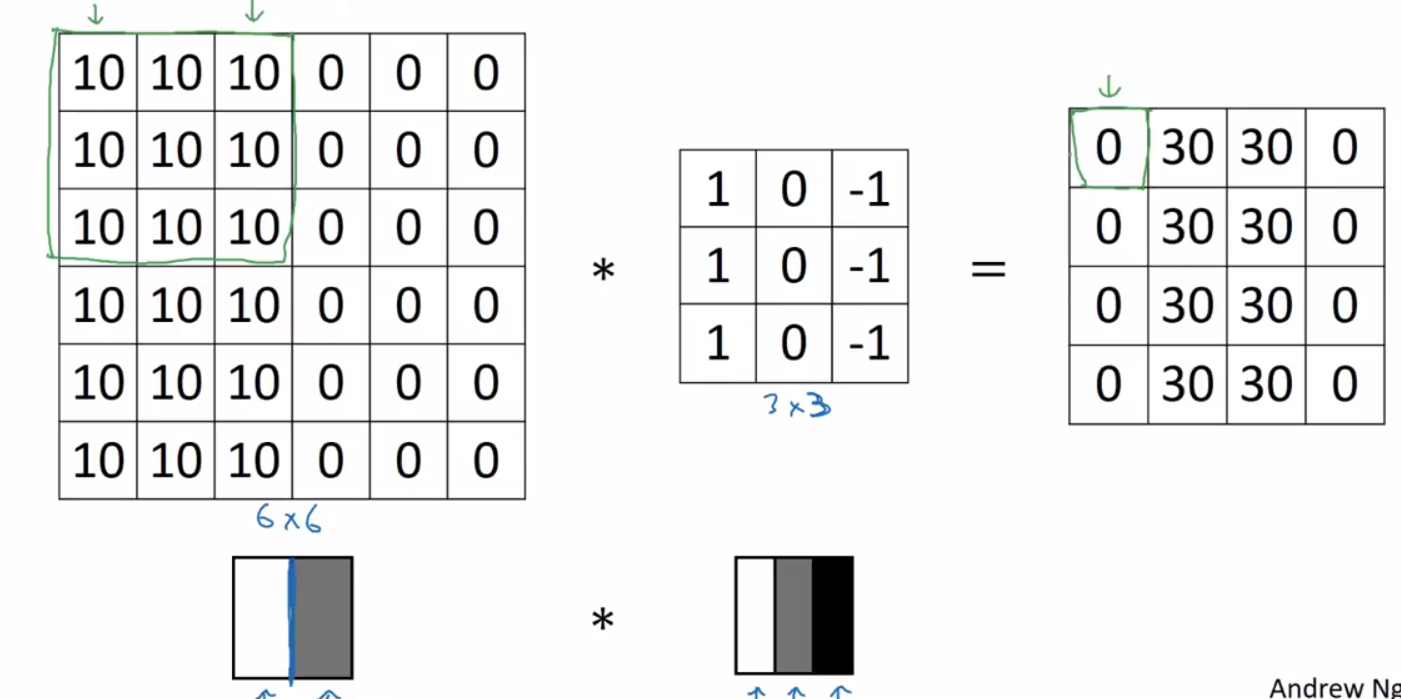
\includegraphics[width=0.6\textwidth]{esempio_convoluzione}
  \label{fig:conv_example}
  \caption{TODO Immagine da rifare}
\end{figure}

\paragraph{Trasformazioni Affini}
% https://en.wikipedia.org/wiki/Digital_image_processing
% https://en.wikipedia.org/wiki/Affine_transformation
% https://en.wikipedia.org/wiki/Rotation

TODO RIEMPIRE DI TEORIA QUA

\paragraph{Feature Extraction}
Come ultima cosa prima di cominciare a descrivere gli algoritmi, si vuole specificare cosa significa \textit{Feature Extraction}.
% https://en.wikipedia.org/wiki/Feature_extraction
% https://deepai.org/machine-learning-glossary-and-terms/feature-extraction
TODO


\clearpage
Ora verranno introdotti alcuni algoritmi fondamentali nel campo della \textit{Computer Vision}.

TODO aggiungere applicazioni principali per ogni tecnica?

TODO sono da riscrivere meglio.


\subsection {Passaggio da RGB a GrayScale}
La conversione di un'immagine da RGB in scala di grigi è un'operazione estremamente facile, ma rimane comunque alla base di molti algoritmi di image processing.
Infatti per molti compiti l'informazione sul colore non è necessaria.
Il modo più semplice per combinare i tre canali RGB in un unico canale è quello di fare la media dei valori pixel per pixel:
\begin{equation}
  Y = (R + G + B)/3
\end{equation}
\label{eq:rgb2gray_avg}
In questo modo ogni canale partecipa allo stesso modo.
Però sappiamo che l'occhio umano è più sensibile ai colori verdi, quindi potrebbe essere preferibile dare più importanza al secondo canale:
\begin{equation}
  Y = 0.299*R + 0.587*G + 0.114*B
\end{equation}
\label{eq:rgb2gray}
I pesi sono stati definiti nello standard CCIR 601.
Il risulato di quest'ultimo calcolo è rappresentato in Figura~\ref{fig:rgb2gray_example}.

% TODO accennare agli altri metodi?
% https://www.johndcook.com/blog/2009/08/24/algorithms-convert-color-grayscale/
% https://docs.opencv.org/3.1.0/de/d25/imgproc_color_conversions.html
% https://stackoverflow.com/questions/19181323/what-grayscale-conversion-algorithm-does-opencv-cvtcolor-use
\begin{figure}[ht]
  \begin{center}
    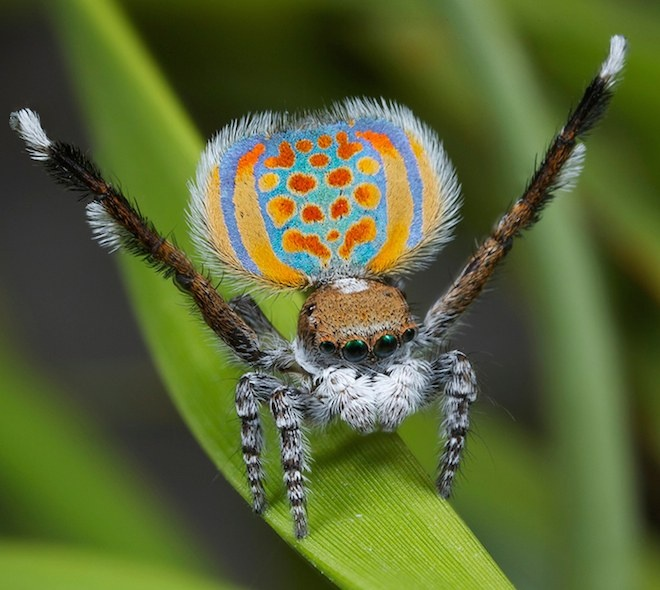
\includegraphics[width=0.3\textwidth]{RGB}
    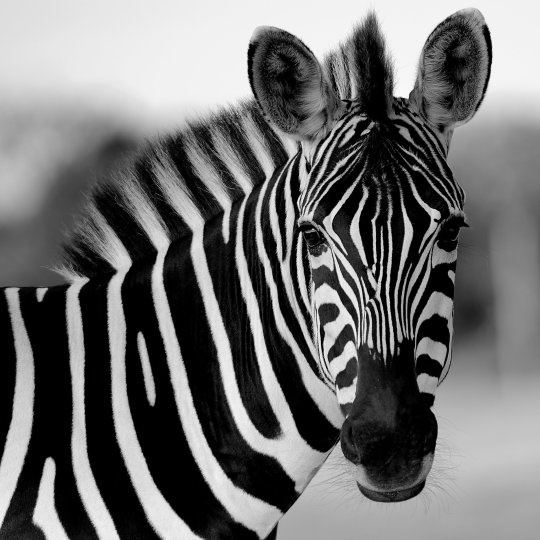
\includegraphics[width=0.3\textwidth]{RGBtoGRAY}
    \label{fig:rgb2gray_example}
    \caption{A sinistra l'immagine originale. A destra la versione in scala di grigi}
  \end{center}
\end{figure}


\clearpage
\subsection {Masking}
La tecnica del masking permette di nascondere parti di immagine a cui non siamo interessati.
Abbiamo bisogno di una maschera binaria, nella quale ogni pixel appartiene all'insieme $\{0,1\}$, che solitamente viene generata a mano, ed ovviamente dell'immagine che si vuole mascherare.
La maschera deve avere le stesse dimensioni dell'immagine di partenza.
L'operazione consiste nell'effettuare un AND logico, pixel per pixel,  tra l'immagine e la maschera.
Così facendo tutti i pixel dell'immagine di partenza corrispondenti a zone di valore $0$ della maschera verranno impostati a $0$, diventando quindi neri.
Il resto dell'immagine rimane con i colori originali.

Nell'esempio in Figura~\ref{fig:mask_example} si è deciso di rimuove l'informazione relativa allo sfondo.
\begin{figure}[ht] % TODO migliorare caption
  \begin{center}
    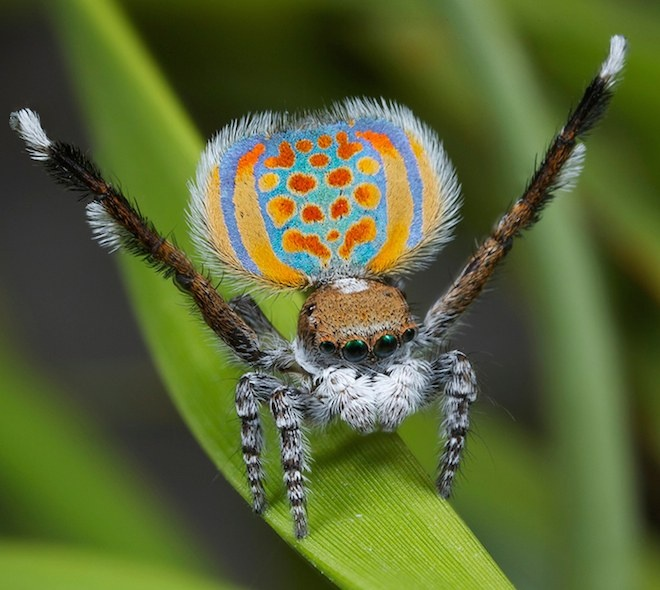
\includegraphics[width=0.3\textwidth]{RGB}
    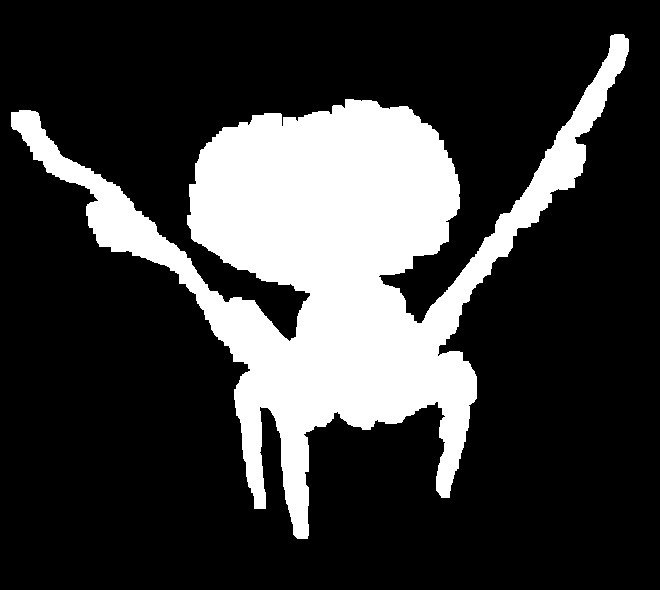
\includegraphics[width=0.3\textwidth]{mask}
    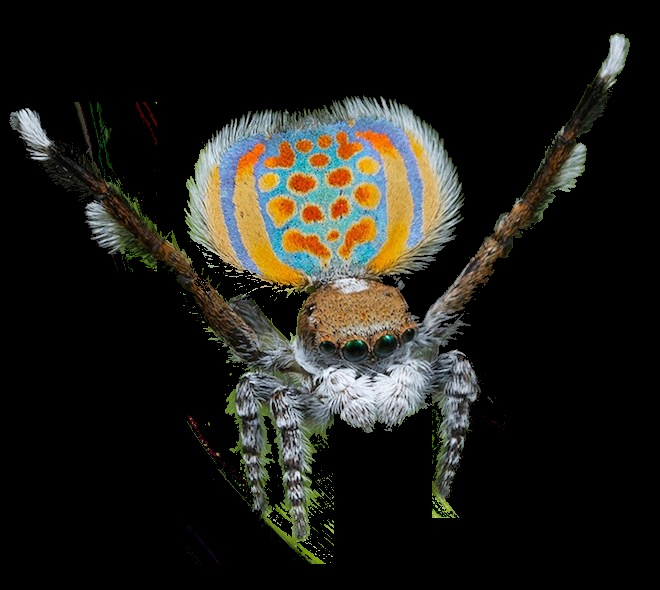
\includegraphics[width=0.3\textwidth]{masked}
    \label{fig:mask_example}
    \caption{Da sinistra a destra: immagine originale, maschera binaria, risultato del masking}
  \end{center}
\end{figure}

% TODO dire che ci sono vari tipi di masking?

\clearpage
\subsection {Traslazioni e Rotazioni}
Come abbiamo accennato prima, le trasformazioni affini ci permettono di effettuare traslazioni e rotazioni alle immagini.

TODOOOOOOO

Con la matrice per il cambio di base hhkk
% wrap affine e matrici di traslazione / rotazione
% cfr cambio di base?
\begin{figure}[ht] % TODO immagini
  \begin{center}
    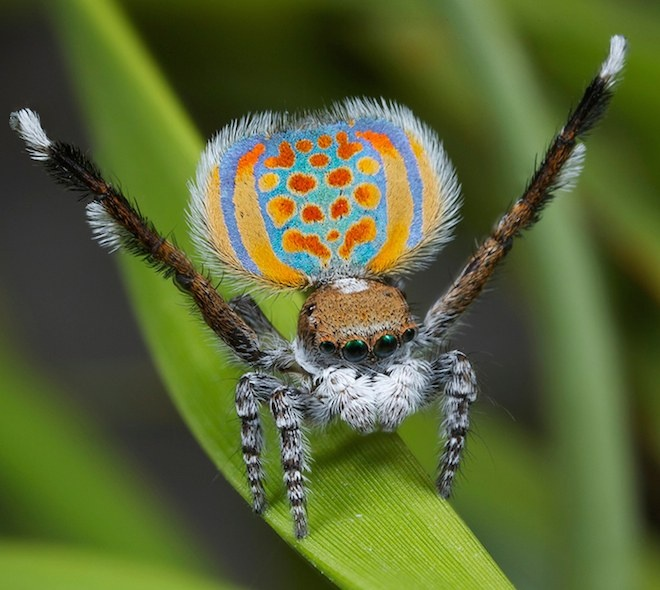
\includegraphics[width=0.3\textwidth]{RGB}
    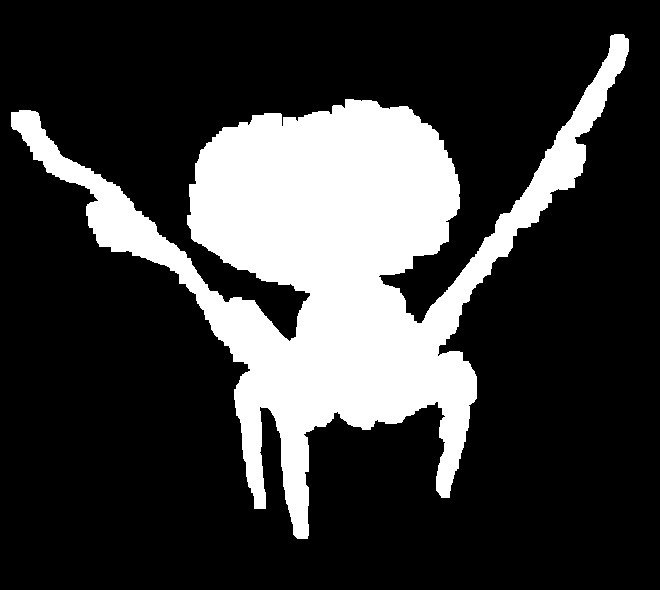
\includegraphics[width=0.2\textwidth]{mask}
    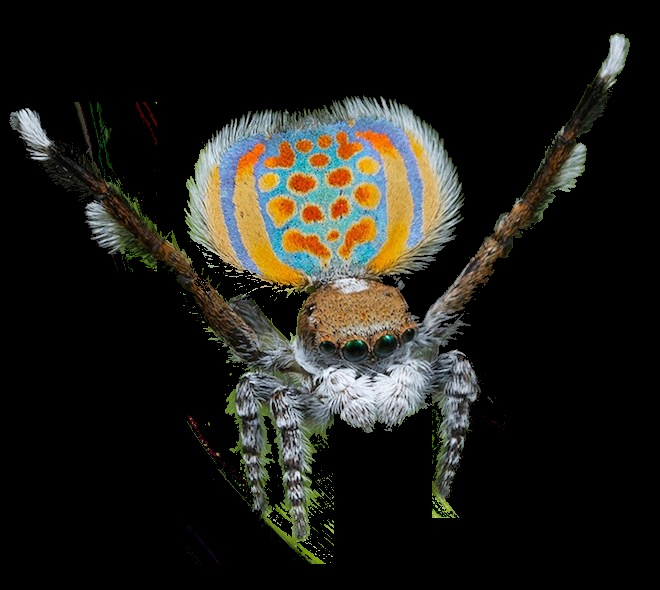
\includegraphics[width=0.3\textwidth]{masked}
    \label{fig:traslation_example}
    \caption{TODO cambiare immagini}
  \end{center}
\end{figure}

\clearpage
\subsection {Image Cropping and Resizing}
Quando si effettua un \textit{image cropping} si ritaglia una porzione dell'immagine, che viene chiamata ROI (\textit{Region Of Interest}), sulla quale vogliamo concentrare la nostra attenzione.
Dato che ogni immagine è rappresentata con una matrice, una ROI non sarà nient'altro che una matrice di dimensioni minori in cui sono stati copiati i valori dell'area interessata.
Una matrice di questo tipo viene anche chiamata \textit{view}.
% https://en.wikipedia.org/wiki/Cropping_(image)

Con l'\textit{image resizing} si aumentano (o diminuiscono) le dimensioni di un'immagine.
Nel primo caso, poiché si vuole aumentare il numero di pixel dell'immagine finale,bisognerà utilizzare tecniche di upsampling ed interpolare i dati a disposizione per generarne di nuovi che siano verosimili.

Uno fra gli algoritmi più semplici è Nearest-Neighbor Interpolation:
il pixel che deve essere aggiunto ottiene il valore del pixel a lui più vicino.
Un criterio di scelta dovrà essere definito nel caso in cui ci siano più pixel alla stessa distanza ma con valori differenti.
Un criterio possibile è quello di assegnare al nuovo pixel sempre il valore del pixel in alto a sinistra.
% https://en.wikipedia.org/wiki/Nearest-neighbor_interpolation
% https://docs.opencv.org/2.4/modules/imgproc/doc/geometric_transformations.html
% https://en.wikipedia.org/wiki/Image_scaling
% https://en.wikipedia.org/wiki/Scale_(ratio)

Una tecnica leggermente più complessa, ma che fornisce risultati soddisfacenti nella maggior parte delle occasioni, è l'interpolazione bilineare.
Con questa tecnica si effettuano, in cascata, due interpolazioni lineari, una orizzontale ed una verticale.
Con l'interpolazione bilineare i nuovi pixel si ottengono come media dei valori noti, pesata rispetto allo loro distanza dal pixel che si vuole colorare.
In questo modo si ottengono immagini con cambi di colore più dolci.

TODO
Parentesi sulle formule?
Linear Interpolation
% https://en.wikipedia.org/wiki/Linear_interpolation
per poi spiegare Bilinear Interpolation?
% https://en.wikipedia.org/wiki/Bilinear_interpolation
%https://theailearner.com/2018/12/29/image-processing-bilinear-interpolation/


Nel caso in cui si voglia ridurre le dimensioni dell'immagine si dovranno usare tecniche di \textit{downsampling} ed \textit{anti-aliasing}.
% https://en.wikipedia.org/wiki/Anti-aliasing_filter
Il downsampling permette di selezionare un numero limitato di pixel che poi verranno usati per colorare la matrice di dimensione ridotta.
Applicare soltanto questa tecnica può portare alla creazione di artefatti sintetici nell'immagine risultato.
Significa che l'immagine ridotta potrebbe contenere gruppi di pixel di colori sbagliati.
Sfruttando tecniche come l'anti-aliasing si può evitare, o quantomeno limitare, la creazione di tali artefatti.
Un \textit{low-pass filter} è un tipo di filtro che smorza tutti i valori al di sopra di una certa soglia, mentre lascia passare tutti i valori minori.
Nel campo del \textit{digital image processing} vengono utilizzati filtri di \textit{blur} applicati tramite convoluzione.
Il termine \textit{blur} o \textit{smooth} indicano applicare un effetto sfuocato che tende a rendere più dolci le transizioni da un colore all'altro, andando quindi anche a ridurre valori troppo alti (o troppo bassi) avvicinandoli a valori più probabili.


\clearpage
\subsection {Histogram Equalization}
Questa tecnica permette di "aggiustare" il contrasto di un'immagine sfruttandone l'istogramma.
Il contrasto è definito come la differenza in intensità luminosa e colore che permette di distinguere gli oggetti.

In Figura~\ref{fig:hist_eq_example} sono stati riporta un'immagine a basso contrasto e l'immagine risultato dopo l'applicazione della \textit{histogram equalization}.
Sotto ogni immagine si possono osservare i relativi istogrammi: sull'asse delle $x$ abbiamo ogni possibile valore di un pixel, quindi da 0 a 255; sull'asse delle $y$ è riportato il numero di occorrenze di quel colore nell'immagine.
Notare che l'immagine in input deve essere in scala di grigi.

Vediamo ora come possiamo formulare matematicamente la costruzione dell'istogramma e la sua manipolazione.
Siano $X$ l'immagine di partenza ed $Y$ l'immagine risultato.
Facendo riferimento a quanto scritto nel documento (TODO AGGIUNGERE REF A DOC) l'istogramma può essere definito come:
\begin{equation*}
p_n = \frac{\text{\# di pixel di colore} \quad n}{\text{\# totale di pixel}} \quad \text{con} \quad n \in [0,255]
\end{equation*}
Poiché $p_n$ descrive la probabilità che un pixel, scelto a caso dall'immagine, abbia valore $n$, possiamo considerare $X$ una variabile casuale discreta in $[0,255]$.
Quindi $X$ avrà funzione di ripartizione, tracciata in nero nel grafico, pari ad:
\begin{equation*}
  F_X(x) = \sum_{n=0}^{x} p_n
\end{equation*}
Noi vorremmo che la differenza di colore tra i pixel fosse più netta, così da aumentare il contrasto dell'immagine.
Per raggiungere i nostri scopi possiamo ridistribuire equamente i valori di $X$ nell'intervallo dei valori possibili:
\begin{equation*}
  T(x) = \text{floor}(255 * F_X(x))
\end{equation*}
dove floor() arrotonda verso il basso all'intero più vicino.
In questo modo possiamo ottenere la variabile casuale trasformata $Y=T(X)$, ossia l'immagine equalizzata.
Sostanzialmente abbiamo ricolorato ogni pixel dell'immagine di partenza con colori più distanti tra loro.

\begin{figure}[ht] % TODO rifare grafici
  \begin{center}
    \begin{tabular}{cc}
      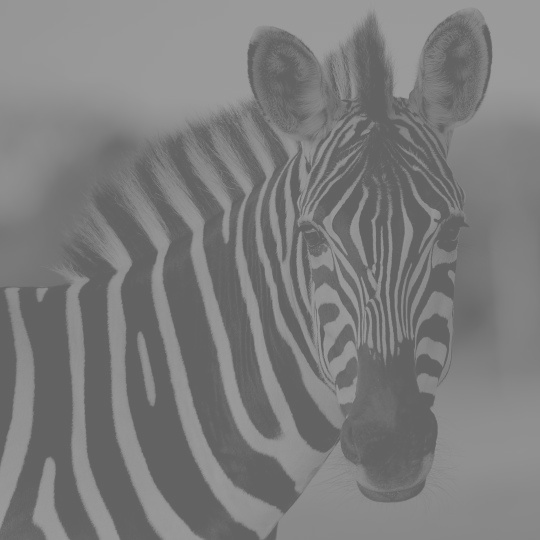
\includegraphics[width=0.3\textwidth]{GRAY_low_contrast} &
      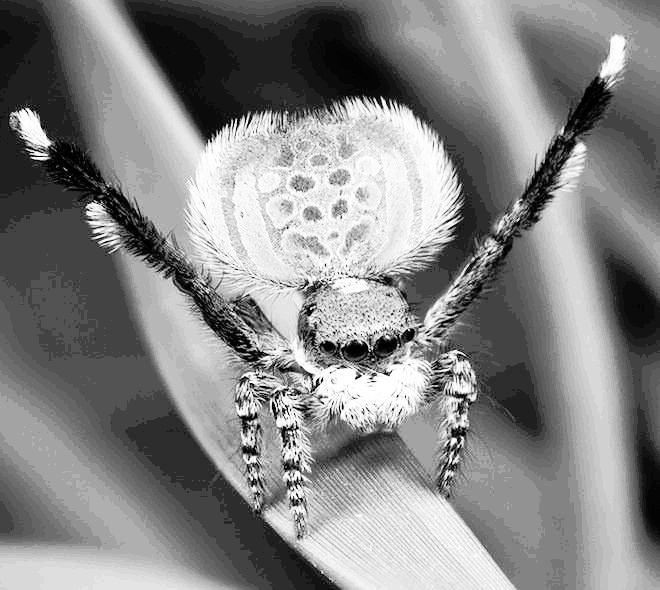
\includegraphics[width=0.3\textwidth]{eqHist_example} \\
      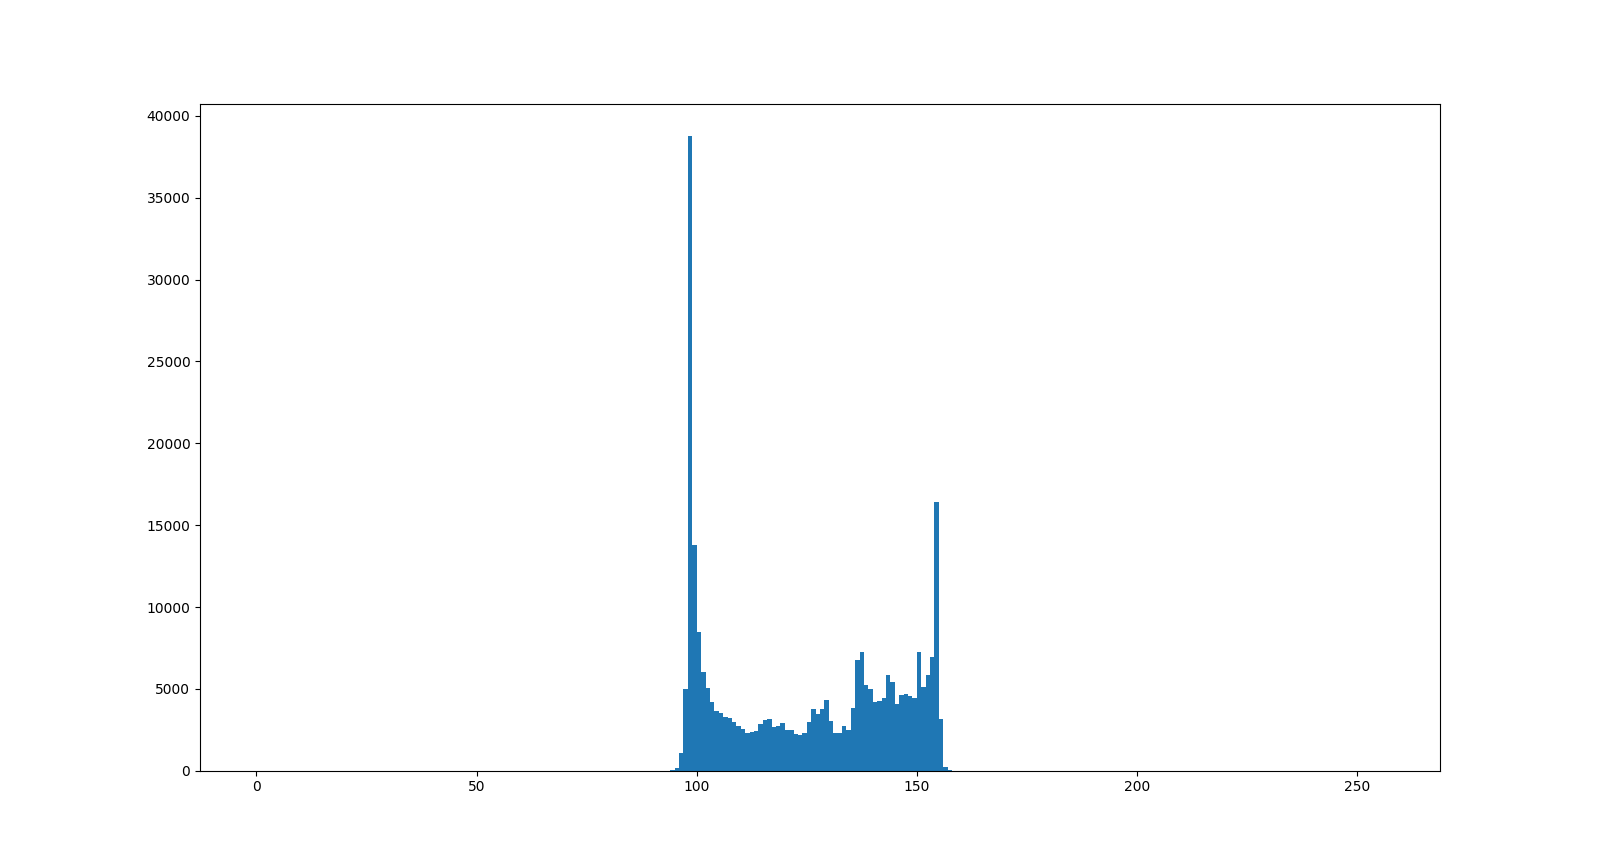
\includegraphics[width=0.3\textwidth]{pre_eq_hist} &
      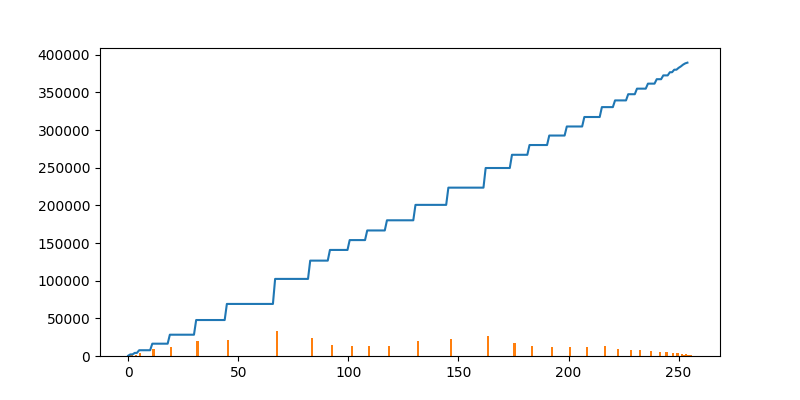
\includegraphics[width=0.3\textwidth]{post_eq_hist}
    \end{tabular}
    \label{fig:hist_eq_example}
    \caption{TODO rifare caption e grafici}
  \end{center}
\end{figure}


% https://en.wikipedia.org/wiki/Histogram_equalization

\clearpage
\subsection {Gaussian Blur}
Conosciuto anche come \textit{Gaussian smoothing}, il \textit{Gaussian blur} permette di sfocare un immagine sfruttando una convoluzione con kernel gaussiano.
L'immagine così ottenuta risulta meno nitida, con meno dettagli e, quindi, con meno rumore.
L'obbiettivo principale di questa tecnica è mantenere soltanto l'informazione caratterizzante, rimuovendo quella non necessaria od anomala.
Si può dimostrare che il \textit{Gaussian blur} è un \textit{low-pass filter}.

Si ricorda che la funzione di Gauss ad un parametro è
\begin{equation*}
  G(x) = \frac{1}{\sqrt{2\pi\sigma^2}}
         \exp{\Bigl(- \frac{ x^2 }{ 2 \sigma^2 } \Bigr)} 
\end{equation*}
Si dimostra che la funzione di Gauss a due parametri equivale al prodotto di due funzioni come quella appena definita, in formule
\begin{equation}
  \begin{split}
    G(x,y) & = G(x)G(y) \\
           & = \frac{1}{2\pi\sigma^2}
               \exp{\Bigl(- \frac{ x^2 + y^2 }{ 2 \sigma^2 } \Bigr)} 
  \end{split}
\end{equation}
in cui $x$ ed $y$ sono le distanze dagli assi di riferimento, mentre $\sigma$ è la deviazione standard.
In termini di calcolo computazionale ciò può essere sfruttato eseguendo due computazioni lineari,
rispetto alle dimensioni dell'immagine e del kernel, %non corretto
anziché una quadratica.

$
{\displaystyle O\left(w_{\text{kernel}}w_{\text{image}}h_{\text{image}}\right)+O\left(h_{\text{kernel}}w_{\text{image}}h_{\text{image}}\right)}
$

$
{\displaystyle O\left(w_{\text{kernel}}h_{\text{kernel}}w_{\text{image}}h_{\text{image}}\right)}
$
TODO correggere e dire meglio.


La matrice sottostante rappresenta un filtro gaussiano quadrato di lato $7$ con $\sigma = 2$.

\begin{equation*} % TODO 
  \begin{bmatrix}
    0&0&0&0&0&0&0\\
    0&0&0&0&0&0&0\\
    0&0&0&0&0&0&0\\
    0&0&0&0&0&0&0\\
    0&0&0&0&0&0&0\\
    0&0&0&0&0&0&0\\
    0&0&0&0&0&0&0
  \end{bmatrix}
\end{equation*}

Ricordiamo che durante una convoluzione si effettua la somma di prodotti elemento per elemento, ossia una media pesata in cui i pesi sono definiti nel kernel.
Dato che i valori al centro del filtro sono più grandi di quelli ai bordi, daremo maggior peso ai pixel nell'intorno dell'elemento su cui il kernel viene centrato.
Sappiamo che all'aumentare di $\sigma$ cresce il raggio alla base della campana di Gauss, questo significa che verrà data sempre più importanza ai pixel distanti.
Ciò farà risultare l'immagine in uscita molto più sfocata.

%\begin{figure}[ht] % TODO
%  \begin{center}
%    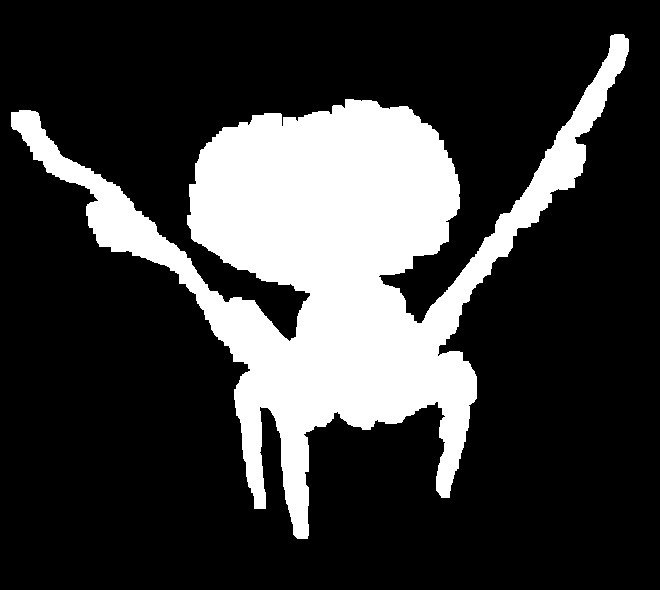
\includegraphics[width=0.3\textwidth]{mask} % plot 3d del kernel
%    \label{fig:gaussian_kernel}
%    \caption{TODO plot 3d del kernel}
%  \end{center}
%\end{figure}

In Figura~\ref{fig:gaussian_blur_example} è riportata un'immagine prima e dopo l'applicazione del filtro appena descritto, si nota come i dettagli più piccoli sono stati rimossi, mentre l'oggetto dell'immagine rimane distinguibile.

\begin{figure}[ht] % TODO
  \begin{center}
    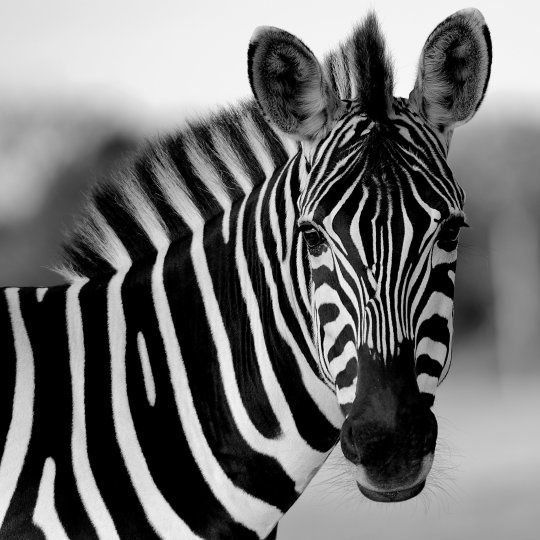
\includegraphics[width=0.3\textwidth]{GRAY}
    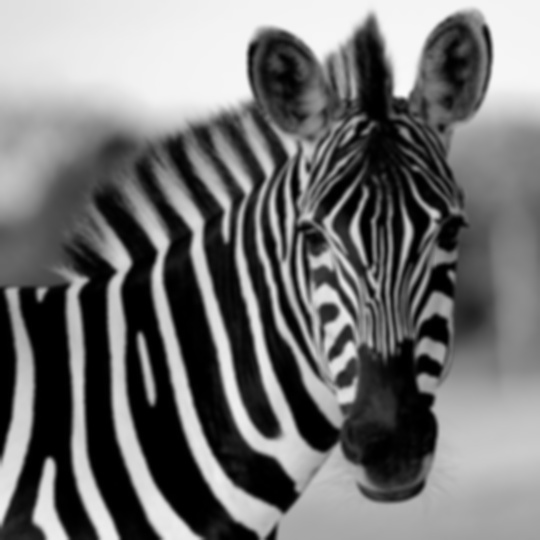
\includegraphics[width=0.3\textwidth]{gaussian_blur_example}
    \label{fig:gaussian_blur_example}
    \caption{TODO rifare caption}
  \end{center}
\end{figure}

Va fatta un'ultima considerazione: COSA SUCCEDE SE APPLICO DUE VOLTE LO STESSO FILTRO?
Se si applica più volte uno stesso filtro gaussiano si ottiene lo stesso risultato che si otterrebbe dopo un'unica applicazione di un filtro 
\fbox{TODO completare}

% https://en.wikipedia.org/wiki/Gaussian_blur

%\clearpage
%\subsection {Bilateral Filter}
%TODO
% https://en.wikipedia.org/wiki/Bilateral_filter
% https://docs.opencv.org/2.4/modules/imgproc/doc/filtering.html?highlight=bilateralfilter#bilateralfilter

% Capire formule in 
% http://homepages.inf.ed.ac.uk/rbf/CVonline/LOCAL_COPIES/MANDUCHI1/Bilateral_Filtering.htmlhttp://homepages.inf.ed.ac.uk/rbf/CVonline/LOCAL_COPIES/MANDUCHI1/Bilateral_Filtering.html


\clearpage
\subsection {Sobel Operator}
Prima di descrivere cosa sia il \textit{Sobel operator}, detto anche \textit{Sobel filter}, bisogna dare una definizione di gradiente.
% TODO formattare correttamente la citazione
Nel calcolo vettoriale, il gradiente è la generalizzazione della derivata.
La derivata di una funzione ad una variabile associa ad ogni punto uno scalare, mentre il gradiente di una funzione $f$ a più variabili associa ad ogni punto un vettore multidimensionale.
Quest'ultimo è composto dall'insieme delle derivate parziali di $f$ nel punto considerato.
Il gradiente rappresenta la pendenza della tangente al grafico della funzione in un punto.
La sua direzione indica il più grande incremento della funzione mentre la magnitudine è il tasso d'incremento.

Possiamo pensare un'immagine (in scala di grigi) come una funzione a due variabili che associa ad ogni punto $(x,y)$ un valore in $[0,255]$.
Il gradiente dell'immagine sarà composto da vettori direzionati in modo da uscire dalle zone scure ed entrare nelle zone più chiare (mantenendo la convenzione per cui a zero è associato il colore nero).
La magnitudine sarà tanto più grande quanto più grande il contrasto, quindi differenza di colore e luminosità.
%In Figura~\ref{fig:gradient} è presentato un esempio di gradiente di un'immagine.
%\begin{figure}[ht] % TODO
%  \begin{center}
%    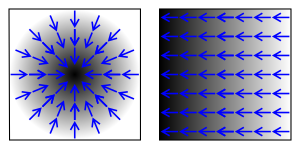
\includegraphics[width=0.2\textwidth]{gradient}
%    \label{fig:gradient}
%    \caption{TODO occhio che qui black=high e white=low}
%  \end{center}
%\end{figure}

Ora possiamo procedere con la descrizione del filtro di Sobel.
Il \textit{Sobel filter} viene utilizzato per creare immagini in cui si enfatizzano gli \textit{edge}.
Per \textit{edge} si intendono tutte quelle zone dell'immagine che corrispondono a bordi, margini o spigoli degli oggetti rappresentati nell'immagine.
Ciascuna di queste zone deve necessariamente essere associata almeno ad un cambio di colore oppure ad un cambio di luminosità, altrimenti l'oggetto in questione non sarebbe distinguibile dallo sfondo.
Quindi, osservando il gradiente dell'immagine, ad ogni \textit{edge} corrisponderà una serie di vettori con magnitudine più grande rispetto alle magnitudini dei vettori circostanti.
Lo scopo del \textit{Sobel operator} è generare una approssimazione del gradiente dell'immagine sfruttando due convoluzioni distinte con uno specifico kernel.
Nonostante il risultato sia abbastanza grossolano, la sua efficacia e rapidità lo rendono uno dei principali strumenti per la \textit{edge detection}, tecnica che esploreremo fra poco.

L'applicazione del filtro Sobel avviene come mostrato nelle due equazioni sottostanti, dove $*$ denota una convoluzione ed $I$ è un'immagine in scala di grigi.

\begin{equation} \label{eq:sobel_gx}
  G_x = 
  I
  *
  \begin{bmatrix}
    -1&0&1\\
    -2&0&2\\
    -1&0&1\\
  \end{bmatrix}
\end{equation}
\begin{equation} \label{eq:sobel_gy}
  G_y = 
  I
  *
  \begin{bmatrix}
    -1&-2&-1\\
    0&0&0\\
    1&2&1\\
  \end{bmatrix}
\end{equation}
\begin{equation} \label{eq:sobel_g}
  G = \sqrt{G_x^2 + G_y^2}
\end{equation}
%\begin{equation} \label{eq:sobel_angle}
%  \Theta = atan{\Bigl( \frac{G_y}{G_x} \Bigr)}
%\end{equation}
% TODO allineare le equazioni

La prima equazione fornisce un'approssimazione del gradiente rispetto all'asse $x$, mentre la seconda rispetto ad $y$.
La terza equazione, invece, combina le precedenti fornendoci informazione riguardo alla magnitudine del gradiente dell'immagine.
%TODO aggiungere anche l'angolo?

Ora verranno fatte delle considerazioni sul primo kernel ma, poiché il secondo è una semplice trasposta del primo, tali considerazioni sono, facendo riferimento all'asse delle $y$, valide anche per il filtro in equazione \ref{eq:sobel_gy}.
Il kernel nell'equazione~\ref{eq:sobel_gx} assegnerà valori in assoluto più grandi a pixel in una posizione di transizione di colore, rispetto a pixel posizionati in una zona con colorazione uniforme.
Prendiamo un pixel $p$ di colore bianco posizionato in una zona in cui tutti i pixel sono di colore bianco, si avrà che il kernel, pesando i pixel a destra allo stesso modo di quelli di sinistra ma con segno opposto, attribuisce un valore pari a $0$ a $p$.
Se $p$ fosse stato in una zona si transizione dal bianco al nero, avrebbe ottenuto un valore negativo molto grande:
tutti i valori nella prima colonna del filtro verrebbero moltiplicati per $255$ mentre tutti quelli dell'ultima colonna verrebbero annullati, essendo moltiplicati per $0$.


Nell'immagine sottostante viene mostrata l'applicazione dell'operatore Sobel prima rispetto ad $x$, poi rispetto ad $y$ ed infine il risultato della combinazione delle precedenti.

\begin{figure}[ht] % TODO
  \begin{center}
    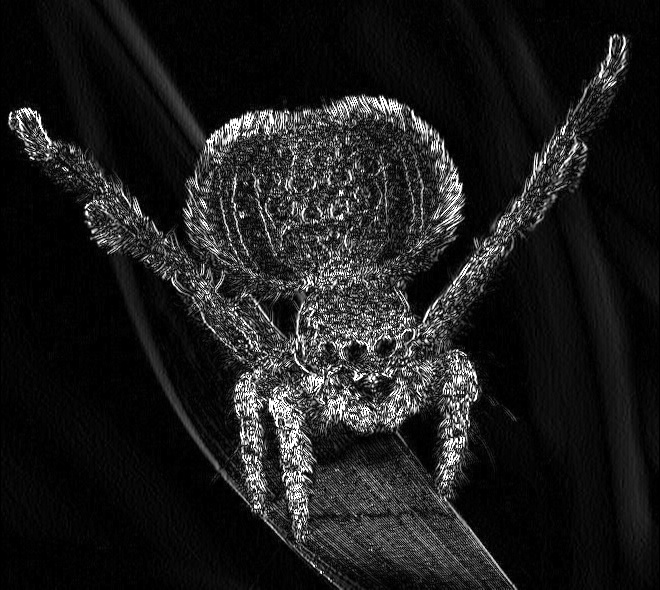
\includegraphics[width=0.3\textwidth]{gx}
    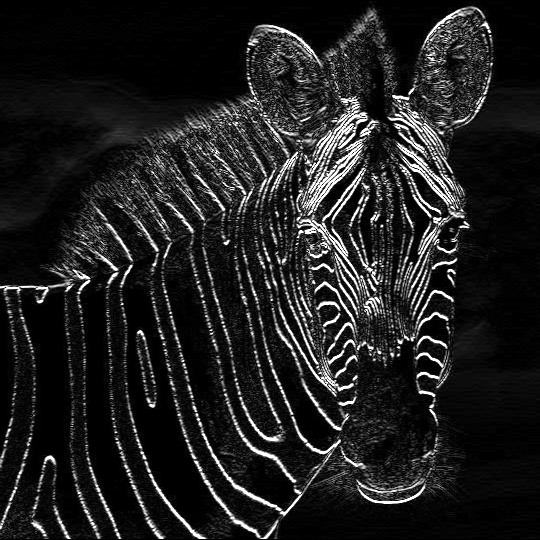
\includegraphics[width=0.3\textwidth]{gy}
    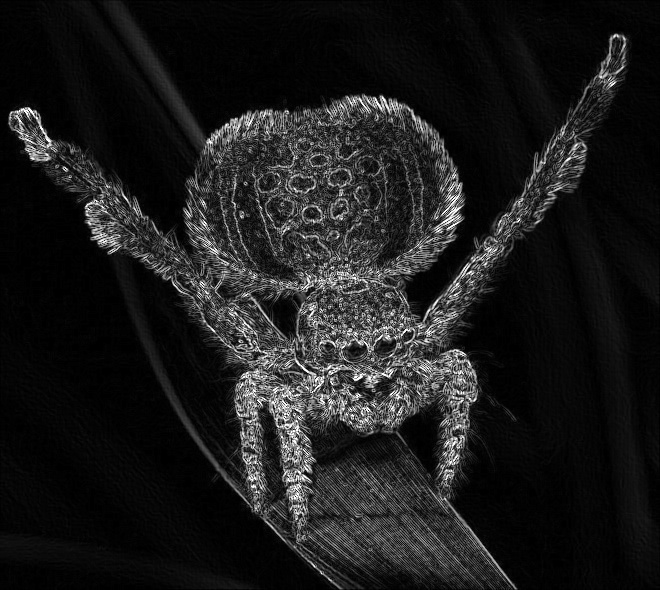
\includegraphics[width=0.3\textwidth]{g}
    \label{fig:sobel_example}
    \caption{TODO caption}
  \end{center}
\end{figure}



% https://en.wikipedia.org/wiki/Sobel_operator
% https://en.wikipedia.org/wiki/Gradient

\clearpage
\subsection {Canny Edge Detector}
Composto da vari passaggi ed algoritmi, il \textit{Canny Edge Detector} permette di estrarre i principali \textit{edge} di un'immagine ottenendo risultati soddisfacenti ed adattabili alle necessità dell'utilizzatore.
Questo rilevatore viene sfruttato largamente come tecnica di \textit{feature extraction} perché permette di rimuovere molta informazione dall'immagine mantenendo solo quella strettamente necessaria.
Nell'ambito del \textit{edge detection} è bene che tutti gli \textit{edge} presenti nell'immagine vengano identificati correttamente, ma è altrettanto importante che non vengano generati falsi positivi, cioè che delle aree nel risultato presentino contorni che nell'immagine di partenza non esistevano.
Per questo motivo \textit{Canny edge detector} effettua molte operazioni di rimozione di falsi positivi ed allo stesso tempo tende ad evidenziare molto bene quelli che sembrano essere \textit{edge autentici}.
Ora verranno elencati in ordine i vari passaggi del rilevatore:
\begin{enumerate}
  \item Viene applicato un filtro gaussiano per effettuare uno \textit{smooth} all'immagine.
    Questo passaggio è fondamentale perché vengono rimossi valori anomali che, risultando come picchi positivi o negativi, potrebbero contribuire a generare falsi positivi.
    Inoltre rimuove può essere usato per rimuovere dettagli superflui.

  \item Utilizzando il \textit{Sobel operator} si ottiene la magnitudine dei gradienti dell'immagine, ossia tutti gli \textit{edge} candidati, che dovranno poi essere manipolati e selezionati.

  %\item Con il \textit{non-maximum suppression}  % TODO fare se c'e spazio

  \item Con una doppia sogliatura si ottengono due effetti:
    come prima cosa vengono rimossi tutti quegli edge con magnitudine troppo bassa, perché considerati rumore;
    successivamente gli edge sopravvissuti vengono classificati come forti e deboli, questa informazione verrà sfruttata nel prossimo passaggio.
    Effettuare una sogliatura significa semplicemente osservare ogni valore di un'immagine, nel nostro caso ogni pixel indica la magnitudine, e mapparlo ad un valore dato se soddisfa determinate condizioni.
    In questo passaggio sono presenti due soglie.
    La prima ci permette di annullare tutti gli edge con valori troppo piccoli.
    Con la seconda viene usata per etichettare i pixel superiori come \textit{strong edge}.
    Tutti i pixel intermedi vengono considerati \textit{weak edge}.

  \item A questo punto si procede con il rimuovere tutti gli edge deboli che non facciamo parte di edge forti.
    Significa che, per ogni pixel etichettato come \textit{weak edge}, vengono osservati gli otto pixel circostanti.
    Se nessuno di questi è uno \textit{strong edge} allora il pixel centrale viene annullato.
    % TODO cfr Connected Componets

\end{enumerate}
Va fatto notare che i valori delle due soglie devono essere trovati in modo empirico, a seconda del tipo d'immagine bisognerà impostare soglie più o meno grandi, ma anche più o meno distanti fra loro.

In Figura~\ref{fig:canny_example} è illustrata l'applicazione del \textit{Sobel operator}, notare come il risultato sia molto più pulito di quello illustro in Figura~\ref{fig:sobel_example}.
\begin{figure}[ht] % TODO
  \begin{center}
    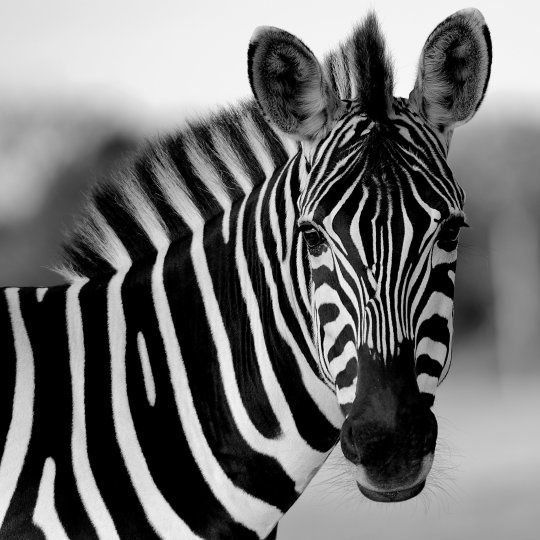
\includegraphics[width=0.3\textwidth]{GRAY}
    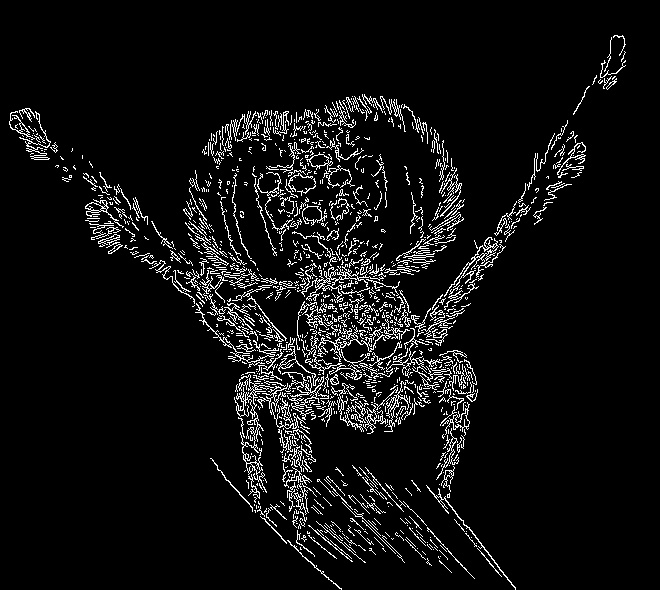
\includegraphics[width=0.3\textwidth]{canny_example}
    \label{fig:canny_example}
    \caption{TODO }
  \end{center}
\end{figure}


% https://en.wikipedia.org/wiki/Canny_edge_detector

\clearpage
\subsection {Hough Circle Transform}
Prima di poter spiegare questa tecnica si devono introdurre alcuni concetti come la \textit{Hough Line Transform}, lo \textit{Hough Parameter Space} e la parametrizzazione raggio-angolo di una retta.
Le trasformate di Hough sono largamente usate come metodi di \textit{feature extraction}, permettono di rilevare semplici figure come linee e cerchi.
Il loro obbiettivo è raggruppare correttamente un'insieme di pixel in modo che l'insieme raffiguri la forma che si vuole trovare.
Una delle problematiche principali è la possibilità che nell'immagine la forma da rilevare sia discontinua o deformata.

Esploriamo come il metodo di \textit{Hough Line Transform} permette di trovare una linea retta in un'immagine.
Definiamo tre punti $P_i=(x_i, x_i)$ con $i=1,2,3$ in modo che siano allineati, cioè che esista una retta a alla quale appartengano tutti.
Sappiamo che per ciascun punto ci sono infinite rette che soddisfano $y_i = m x_i + c$, ma che soltanto una di queste rette passa anche per gli altri due punti.
L'equazione appena descritta è in funzione di $m$ e $c$, riscrivendola come
\begin{equation} \label{eq:cm_lines}
  c = y_i - m x_i \quad con \quad i=1,2,3
\end{equation}
risulta più facile immaginarla (fissato un $i$) come una retta in uno spazio in cui $c$ è sull'asse delle ordinate e $m$ su quello delle ascisse.
Lo spazio appena descritto prende il nome di \textit{Hough Parameter Space}, in cui ogni punto $(m,c)$ descrive una retta nello spazio di partenza.
Nello \textit{Hough Parameter Space} le tre rette della formula \ref{eq:cm_lines} si devono necessariamente incontrarsi in esattamente un punto, sia $(m_0,c_0)$, perché sappiamo che deve esistere una coppia di parametri per cui la retta $y = m_0 x + c_0$, nello spazio originale, passa per tutti gli $P_i$.
L'idea alla base di \textit{Hough Line Transform} è quella di, definito un range di valori per $m$ e per $c$, trovare quello che soddisfa il maggior numero di equazioni.
In pratica ad ogni cella nello spazio $m$-$c$ viene associato un intero che indica quante delle rette di equazione~\ref{eq:cm_lines} ref passano per quella cella.

Ci si accorge facilmente che questo metodo non ci permette di rilevare rette parallele all'asse delle $y$, infatti bisognerebbe avere un parametro $m$ con valore che tende all'infinito.
Per risolvere questa problematica viene usata la parametrizzazione raggio-angolo.
Come si vede in figura~\ref{fig:hough_parametr_raggio-angolo}, ogni retta viene identificata da una coppia univoca $(r,\theta)$.
Nella coppia $r$ indica la distanza dall'origine al punto più vicino della retta, mentre $\theta$ indica l'angolo tra il segmento appena generato e l'asse delle $x$.
Ogni retta viene identificata dall'equazione:
\begin{equation} \label{eq:raggio_angolo_parametr}
  r = x_i cos \theta + y_i sin \theta \quad con \quad i=1,2,3
\end{equation}
ottenibile con semplici calcoli geometrici.
Questo significa che il fascio di rette nello spazio di partenza verrà descritto da curve nello \textit{Hough Parameter Space} $\theta$-$r$, come si vede in figura~TODO.
Valutando le celle nello stesso modo di prima si ottiene la retta passante per i tre punti ma identificata dalla coppia $(r_0,\theta_0)$.

\begin{figure}[ht] % TODO
  \begin{center}
    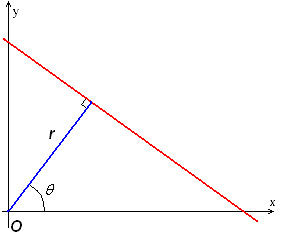
\includegraphics[width=0.3\textwidth]{raggio_angolo}
    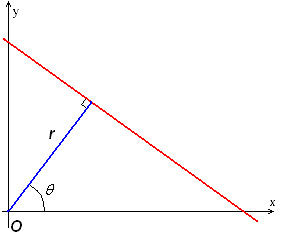
\includegraphics[width=0.3\textwidth]{raggio_angolo}
    \label{fig:hough_parametr_raggio-angolo}
    \caption{TODO }
  \end{center}
\end{figure}


Vediamo ora come si può modificare la tecnica appena descritta per rilevare cerchi anziché linee rette.
L'idea principale ruota sempre attorno al concetto di voto di celle nello spazio di parametri.

In questo caso si sfrutta il fatto che, in una circonferenza $c$ di raggio $r$, ogni punto è equidistante dal centro.
Per ogni punto $P_i$ di $c$ può essere tracciata una circonferenza $c_i$ di centro $P_i$ e raggio $r$.
Sappiamo che tutte le circonferenze $c_i$ si incontrano in un unico punto, il centro di $c$, perché è l'unico equidistante da tutti i centri delle $c_i$.

Si ricorda che l'equazione di una circonferenza di centro $(a,b)$ e raggio $r$ è
\begin{equation} \label{eq:circonferenza}
  (x - a)^2 + (y - b)^2 = r^2
\end{equation}
Supponiamo di conoscere il raggio $r_0$ della circonferenza che vogliamo rilevare e di avere un insieme di punti $P_i$ che sappiamo appartenere alla circonferenza.
Lo spazio dei parametri $a$-$b$ ci permette di creare le circonferenze centrate nei $P_i$ e di assegnare un punteggio alto alla cella in $(a_0,b_0)$ perché votata da molte circonferenze.

Se anche il raggio fosse incognito allora lo \textit{Hough Parameter Space} avrebbe tre dimensioni ed ogni punto sarebbe una tripla $(a,b,r)$ appartenente alla superficie di un cono.
In figura~TODO è illustrata una rappresentazione di questo spazio.

Le implementazioni della \textit{Hough Circle Transform} sfruttano una matrice di supporto, chiamata accumulatore, che corrisponde allo spazio dei parametri di Hough.
Ciascun elemento è un intero con valore iniziale zero, che verrà incrementato di uno per ogni linea passante.

% TODO commento sulla implementazione 
% - immagine deve essere canny edge
% - threshold per fare pochi FP
% - min e max radius per restringere la ricerca


% Risorse
% https://docs.opencv.org/2.4/doc/tutorials/imgproc/imgtrans/hough_circle/hough_circle.html
% https://en.wikipedia.org/wiki/Hough_transform
% https://en.wikipedia.org/wiki/Circle_Hough_Transform

\clearpage
\subsection {Applicazione degli algoritmi descritti}
Si fa notare che prima di ottenere immagini come quella illustrata in Figura~\ref{fig:prima_dopo_prep} e soprattutto prima di essere sicuri che questo è il tipo di immagine migliore per i nostri scopi, sono stati necessari numerosi esperimenti e tentativi.
In particolar modo è stato importante capire che tipo di informazione potesse essere gestita interamente dalla rete neurale e quale invece dovesse essere rimossa o modificata.
Lo scopo del nostro \textit{pre-processing} è quello di fornire un'immagine contenente solo l'informazione necessaria e sufficiente per poter discriminare un pezzo conforme da uno scarto.

Nonostante in questa sezione vengano mostrate solo immagini di carcasse conformi, il processo iterativo appena descritto è stato eseguito confrontando costantemente immagini conformi e scarto.
Immagini scarto verranno mostrate nella prossima sezione, interamente dedicata a loro.

% https://tex.stackexchange.com/questions/343605/latex-code-for-subcaption-of-image
\begin{figure}[ht] % TODO
  \begin{center}
    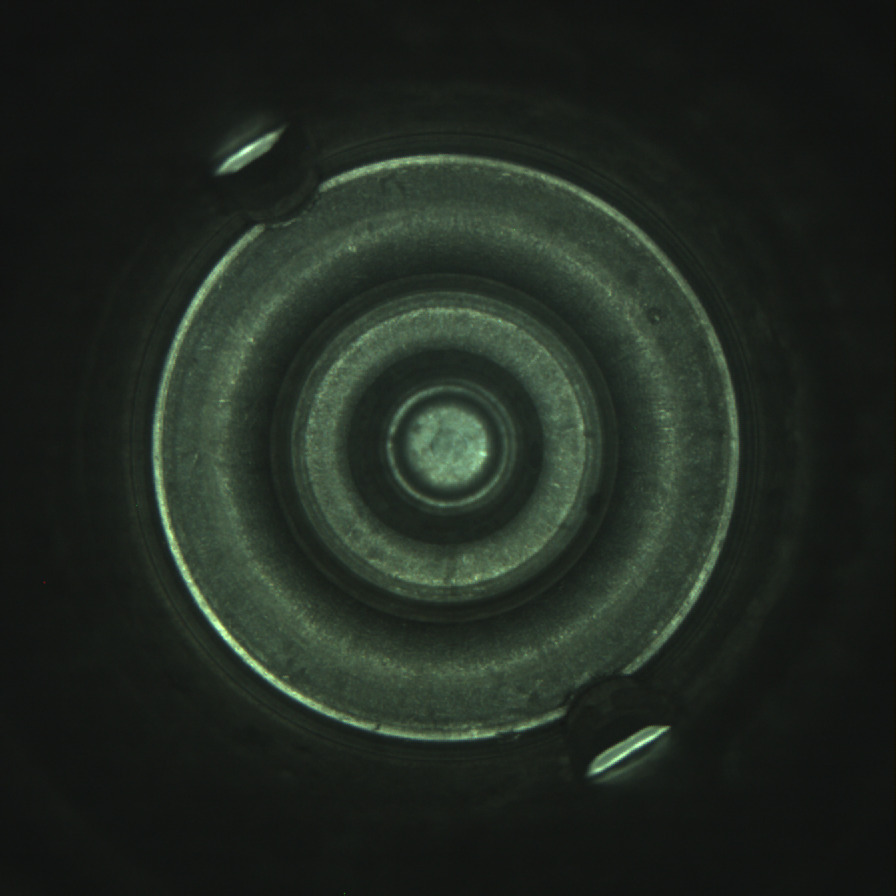
\includegraphics[width=0.5\textwidth]{128___1362_1_1_1_OnLineAnalysis}
    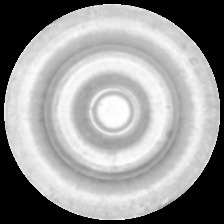
\includegraphics[width=0.35\textwidth]{128___1362_1_1_1_OnLineAnalysis_prep}
    \label{fig:prima_dopo_prep}
    \caption{TODO }
  \end{center}
\end{figure}

\clearpage
Ora verrà illustrato l'ordine in cui sono stati applica gli algoritmi descritti precedentemente e i principali motivi per cui sono stati scelti.

\subsubsection{1 Centramento con Hough Circle Transform}
Sappiamo che le immagini del dataset non sono perfettamente centrate, per questo motivo si è deciso di utilizzare la tecnica della \textit{Hough Circle Transform} per ottenere un'approssimazione del centro della carcassa.
Avendo le coordinate di quest'ultimo si può ottenere una matrice di traslazione con cui riallineare il pezzo con il centro dell'immagine.
% TODO si può specificare che l'immagine deve essere
% - To Grayscale
% - Equalization Histogram
% - ottenere i cerchi con Hough Circle
% - media tra centri
% - trasformazione affine
% - l'immagine uscita è ancora a colori

Nella Figura~\ref{fig:centramento} sono illustrati, a sinistra, il cerchio rilevato, mentre sulla destra l'immagine prima e dopo il centramento.
\begin{figure}[ht] % TODO
  \begin{center}
    \includegraphics[width=0.3\textwidth]{example-image}
    \includegraphics[width=0.3\textwidth]{example-image}
    \includegraphics[width=0.3\textwidth]{example-image}
    \label{fig:centramento}
    \caption{TODO }
  \end{center}
\end{figure}

\subsubsection{2 Equalizzazione}
Per gestire la variazione di luminosità tra immagini si utilizza \textit{equalization histogram}.
In questo modo le immagini in bianco e nero delle carcasse risultano molto più simili tra di loro e si vanno a mitigare i fastidiosi effetti di sovra illuminazione.

D'ora in poi verranno manipolate immagini in scala di grigi.
Questa scelta, validata dagli esperimenti, nasce principalmente dalla prossima considerazione.
Le immagini sono in falsi colori, manterremmo informazione non reale ma soprattutto richiederemmo alla nostra rete neurale uno sforzo molto maggiore.
La rete, infatti, dovrebbe imparare a gestire non solo le forme geometriche del pezzo ma anche le sue colorazioni.

Nella Figura~\ref{fig:equalizzazione} sono illustrate due carcasse conformi con luminosità differenti, affiancate dalla loro trasformazione.
% TODO mostrare l'immagine gray scale prima e dopo
\begin{figure}[ht] % TODO
  \begin{center}
    \begin{tabular}{cc}
      \includegraphics[width=0.3\textwidth]{example-image} &
      \includegraphics[width=0.3\textwidth]{example-image} \\
      \includegraphics[width=0.3\textwidth]{example-image} &
      \includegraphics[width=0.3\textwidth]{example-image}
    \end{tabular}
    \label{fig:equalizzazione}
    \caption{TODO}
  \end{center}
\end{figure}

% TODO si può specificare che l'immagine deve essere
% - To Grayscale
% - Equalization Histogram

\subsubsection{3 Smooth dell'immagine}
Utilizzando un filtro gaussiano è stato rimosso il rumore principale, ossi quello dovuto a graffi ed effetto "sale e pepe".
È stato fondamentale definire il filtro in modo che non fosse troppo aggressivo altrimenti si sarebbe rischiato di perdere l'informazione della colla.

In Figura~\ref{fig:smooth} si mostra l'effetto dell'applicazione del kernel.
% TODO mostrare anche cosa succede se si esagera col filtro?
\begin{figure}[ht] % TODO
  \begin{center}
    \includegraphics[width=0.3\textwidth]{example-image}
    \includegraphics[width=0.3\textwidth]{example-image}
    \label{fig:smooth}
    \caption{TODO}
  \end{center}
\end{figure}

\subsubsection{4 Mascheramento}
L'area che nell'immagine corrisponde alla parete verticale della carcassa, ed in particolar modo alle due balze, deve essere rimossa.
Come abbiamo già sottolineato precedentemente la posizione delle balze non è correlata con la presenza della colla.
Mentre si suppone che la colla non si presenti soltanto sulla parete verticale, ma che coli almeno fino a raggiungere il gradino più ampio.

Nella Figura~\ref{fig:mask} è illustrato un conforme prima e dopo il mascheramento.
Fra le due immagini si presenta la maschera utilizzata.
% TODO mostrare anche cosa succede se si esagera col filtro?
\begin{figure}[ht] % TODO
  \begin{center}
    \includegraphics[width=0.3\textwidth]{example-image}
    \includegraphics[width=0.3\textwidth]{example-image}
    \includegraphics[width=0.3\textwidth]{example-image}
    \label{fig:mask}
    \caption{TODO}
  \end{center}
\end{figure}

\subsubsection{5 Crop e Resizing}
A questo punto l'immagine contiene una grande porzione 
%- crop per levare l'area nera (in proporzione ho molta più informazione)




\clearpage
\section {Data Augmentation}
% Com'è stato sfruttato la Data Aug
% Colle sintetiche
Due metodi principali:
 - rotazione
 - generazione degli scarti sintetici

\subsection {Generazione Scarti Sintetici}


Scarti Sintetici
 I ritagli non sono stati semplicemente incollati sui conformi:

 la luminosità della colla è stata modificata per avvicinarsi a quella del pezzo conforme;
 dopo aver aggiunto la colla è stato praticato uno smooth lungo il contorno, per evitare che ci fosse una transizione netta fra sofndo ed inizio bordo della colla.







































% TODO in caso sarebe un Chapter a sé
%\section {La strada proposta}
% Simile a quanto detto in considerazioni_pixelwise_diff
%Mostrare qual'è l'obbiettivo che si vuole raggiungere con gli AE
%Spiegare che sono elastici e facili da allenare
%Il dataset non richiede dispendioso labeling
